% Options for packages loaded elsewhere
\PassOptionsToPackage{unicode}{hyperref}
\PassOptionsToPackage{hyphens}{url}
\PassOptionsToPackage{dvipsnames,svgnames,x11names}{xcolor}
%
\documentclass[
  11pt,
  a4paper,
]{article}

\usepackage{amsmath,amssymb}
\usepackage[]{libertinus}
\usepackage{iftex}
\ifPDFTeX
  \usepackage[T1]{fontenc}
  \usepackage[utf8]{inputenc}
  \usepackage{textcomp} % provide euro and other symbols
\else % if luatex or xetex
  \usepackage{unicode-math}
  \defaultfontfeatures{Scale=MatchLowercase}
  \defaultfontfeatures[\rmfamily]{Ligatures=TeX,Scale=1}
  \setmonofont[Scale=0.92]{Latin Modern Mono}
\fi
% Use upquote if available, for straight quotes in verbatim environments
\IfFileExists{upquote.sty}{\usepackage{upquote}}{}
\IfFileExists{microtype.sty}{% use microtype if available
  \usepackage[]{microtype}
  \UseMicrotypeSet[protrusion]{basicmath} % disable protrusion for tt fonts
}{}
\makeatletter
\@ifundefined{KOMAClassName}{% if non-KOMA class
  \IfFileExists{parskip.sty}{%
    \usepackage{parskip}
  }{% else
    \setlength{\parindent}{0pt}
    \setlength{\parskip}{6pt plus 2pt minus 1pt}}
}{% if KOMA class
  \KOMAoptions{parskip=half}}
\makeatother
\usepackage{xcolor}
\usepackage[a4paper]{geometry}
\setlength{\emergencystretch}{3em} % prevent overfull lines
\setcounter{secnumdepth}{5}
% Make \paragraph and \subparagraph free-standing
\ifx\paragraph\undefined\else
  \let\oldparagraph\paragraph
  \renewcommand{\paragraph}[1]{\oldparagraph{#1}\mbox{}}
\fi
\ifx\subparagraph\undefined\else
  \let\oldsubparagraph\subparagraph
  \renewcommand{\subparagraph}[1]{\oldsubparagraph{#1}\mbox{}}
\fi

\usepackage{color}
\usepackage{fancyvrb}
\newcommand{\VerbBar}{|}
\newcommand{\VERB}{\Verb[commandchars=\\\{\}]}
\DefineVerbatimEnvironment{Highlighting}{Verbatim}{commandchars=\\\{\}}
% Add ',fontsize=\small' for more characters per line
\newenvironment{Shaded}{}{}
\newcommand{\AlertTok}[1]{\textcolor[rgb]{1.00,0.33,0.33}{\textbf{#1}}}
\newcommand{\AnnotationTok}[1]{\textcolor[rgb]{0.42,0.45,0.49}{#1}}
\newcommand{\AttributeTok}[1]{\textcolor[rgb]{0.84,0.23,0.29}{#1}}
\newcommand{\BaseNTok}[1]{\textcolor[rgb]{0.00,0.36,0.77}{#1}}
\newcommand{\BuiltInTok}[1]{\textcolor[rgb]{0.84,0.23,0.29}{#1}}
\newcommand{\CharTok}[1]{\textcolor[rgb]{0.01,0.18,0.38}{#1}}
\newcommand{\CommentTok}[1]{\textcolor[rgb]{0.42,0.45,0.49}{#1}}
\newcommand{\CommentVarTok}[1]{\textcolor[rgb]{0.42,0.45,0.49}{#1}}
\newcommand{\ConstantTok}[1]{\textcolor[rgb]{0.00,0.36,0.77}{#1}}
\newcommand{\ControlFlowTok}[1]{\textcolor[rgb]{0.84,0.23,0.29}{#1}}
\newcommand{\DataTypeTok}[1]{\textcolor[rgb]{0.84,0.23,0.29}{#1}}
\newcommand{\DecValTok}[1]{\textcolor[rgb]{0.00,0.36,0.77}{#1}}
\newcommand{\DocumentationTok}[1]{\textcolor[rgb]{0.42,0.45,0.49}{#1}}
\newcommand{\ErrorTok}[1]{\textcolor[rgb]{1.00,0.33,0.33}{\underline{#1}}}
\newcommand{\ExtensionTok}[1]{\textcolor[rgb]{0.84,0.23,0.29}{\textbf{#1}}}
\newcommand{\FloatTok}[1]{\textcolor[rgb]{0.00,0.36,0.77}{#1}}
\newcommand{\FunctionTok}[1]{\textcolor[rgb]{0.44,0.26,0.76}{#1}}
\newcommand{\ImportTok}[1]{\textcolor[rgb]{0.01,0.18,0.38}{#1}}
\newcommand{\InformationTok}[1]{\textcolor[rgb]{0.42,0.45,0.49}{#1}}
\newcommand{\KeywordTok}[1]{\textcolor[rgb]{0.84,0.23,0.29}{#1}}
\newcommand{\NormalTok}[1]{\textcolor[rgb]{0.14,0.16,0.18}{#1}}
\newcommand{\OperatorTok}[1]{\textcolor[rgb]{0.14,0.16,0.18}{#1}}
\newcommand{\OtherTok}[1]{\textcolor[rgb]{0.44,0.26,0.76}{#1}}
\newcommand{\PreprocessorTok}[1]{\textcolor[rgb]{0.84,0.23,0.29}{#1}}
\newcommand{\RegionMarkerTok}[1]{\textcolor[rgb]{0.42,0.45,0.49}{#1}}
\newcommand{\SpecialCharTok}[1]{\textcolor[rgb]{0.00,0.36,0.77}{#1}}
\newcommand{\SpecialStringTok}[1]{\textcolor[rgb]{0.01,0.18,0.38}{#1}}
\newcommand{\StringTok}[1]{\textcolor[rgb]{0.01,0.18,0.38}{#1}}
\newcommand{\VariableTok}[1]{\textcolor[rgb]{0.89,0.38,0.04}{#1}}
\newcommand{\VerbatimStringTok}[1]{\textcolor[rgb]{0.01,0.18,0.38}{#1}}
\newcommand{\WarningTok}[1]{\textcolor[rgb]{1.00,0.33,0.33}{#1}}

\providecommand{\tightlist}{%
  \setlength{\itemsep}{0pt}\setlength{\parskip}{0pt}}\usepackage{longtable,booktabs,array}
\usepackage{calc} % for calculating minipage widths
% Correct order of tables after \paragraph or \subparagraph
\usepackage{etoolbox}
\makeatletter
\patchcmd\longtable{\par}{\if@noskipsec\mbox{}\fi\par}{}{}
\makeatother
% Allow footnotes in longtable head/foot
\IfFileExists{footnotehyper.sty}{\usepackage{footnotehyper}}{\usepackage{footnote}}
\makesavenoteenv{longtable}
\usepackage{graphicx}
\makeatletter
\def\maxwidth{\ifdim\Gin@nat@width>\linewidth\linewidth\else\Gin@nat@width\fi}
\def\maxheight{\ifdim\Gin@nat@height>\textheight\textheight\else\Gin@nat@height\fi}
\makeatother
% Scale images if necessary, so that they will not overflow the page
% margins by default, and it is still possible to overwrite the defaults
% using explicit options in \includegraphics[width, height, ...]{}
\setkeys{Gin}{width=\maxwidth,height=\maxheight,keepaspectratio}
% Set default figure placement to htbp
\makeatletter
\def\fps@figure{htbp}
\makeatother
\newlength{\cslhangindent}
\setlength{\cslhangindent}{1.5em}
\newlength{\csllabelwidth}
\setlength{\csllabelwidth}{3em}
\newlength{\cslentryspacingunit} % times entry-spacing
\setlength{\cslentryspacingunit}{\parskip}
\newenvironment{CSLReferences}[2] % #1 hanging-ident, #2 entry spacing
 {% don't indent paragraphs
  \setlength{\parindent}{0pt}
  % turn on hanging indent if param 1 is 1
  \ifodd #1
  \let\oldpar\par
  \def\par{\hangindent=\cslhangindent\oldpar}
  \fi
  % set entry spacing
  \setlength{\parskip}{#2\cslentryspacingunit}
 }%
 {}
\usepackage{calc}
\newcommand{\CSLBlock}[1]{#1\hfill\break}
\newcommand{\CSLLeftMargin}[1]{\parbox[t]{\csllabelwidth}{#1}}
\newcommand{\CSLRightInline}[1]{\parbox[t]{\linewidth - \csllabelwidth}{#1}\break}
\newcommand{\CSLIndent}[1]{\hspace{\cslhangindent}#1}

\usepackage{tikz}
\usepackage{xcolor}
\usepackage{tabularx}
\makeatletter
\@ifpackageloaded{tcolorbox}{}{\usepackage[many]{tcolorbox}}
\@ifpackageloaded{fontawesome5}{}{\usepackage{fontawesome5}}
\definecolor{quarto-callout-color}{HTML}{909090}
\definecolor{quarto-callout-note-color}{HTML}{0758E5}
\definecolor{quarto-callout-important-color}{HTML}{CC1914}
\definecolor{quarto-callout-warning-color}{HTML}{EB9113}
\definecolor{quarto-callout-tip-color}{HTML}{00A047}
\definecolor{quarto-callout-caution-color}{HTML}{FC5300}
\definecolor{quarto-callout-color-frame}{HTML}{acacac}
\definecolor{quarto-callout-note-color-frame}{HTML}{4582ec}
\definecolor{quarto-callout-important-color-frame}{HTML}{d9534f}
\definecolor{quarto-callout-warning-color-frame}{HTML}{f0ad4e}
\definecolor{quarto-callout-tip-color-frame}{HTML}{02b875}
\definecolor{quarto-callout-caution-color-frame}{HTML}{fd7e14}
\makeatother
\makeatletter
\makeatother
\makeatletter
\makeatother
\makeatletter
\@ifpackageloaded{caption}{}{\usepackage{caption}}
\AtBeginDocument{%
\ifdefined\contentsname
  \renewcommand*\contentsname{Table of contents}
\else
  \newcommand\contentsname{Table of contents}
\fi
\ifdefined\listfigurename
  \renewcommand*\listfigurename{List of Figures}
\else
  \newcommand\listfigurename{List of Figures}
\fi
\ifdefined\listtablename
  \renewcommand*\listtablename{List of Tables}
\else
  \newcommand\listtablename{List of Tables}
\fi
\ifdefined\figurename
  \renewcommand*\figurename{Figure}
\else
  \newcommand\figurename{Figure}
\fi
\ifdefined\tablename
  \renewcommand*\tablename{Table}
\else
  \newcommand\tablename{Table}
\fi
}
\@ifpackageloaded{float}{}{\usepackage{float}}
\floatstyle{ruled}
\@ifundefined{c@chapter}{\newfloat{codelisting}{h}{lop}}{\newfloat{codelisting}{h}{lop}[chapter]}
\floatname{codelisting}{Listing}
\newcommand*\listoflistings{\listof{codelisting}{List of Listings}}
\usepackage{amsthm}
\theoremstyle{plain}
\newtheorem{theorem}{Theorem}[section]
\theoremstyle{remark}
\AtBeginDocument{\renewcommand*{\proofname}{Proof}}
\newtheorem*{remark}{Remark}
\newtheorem*{solution}{Solution}
\makeatother
\makeatletter
\@ifpackageloaded{caption}{}{\usepackage{caption}}
\@ifpackageloaded{subcaption}{}{\usepackage{subcaption}}
\makeatother
\makeatletter
\@ifpackageloaded{tcolorbox}{}{\usepackage[many]{tcolorbox}}
\makeatother
\makeatletter
\@ifundefined{shadecolor}{\definecolor{shadecolor}{rgb}{.97, .97, .97}}
\makeatother
\makeatletter
\makeatother
\ifLuaTeX
  \usepackage{selnolig}  % disable illegal ligatures
\fi
\IfFileExists{bookmark.sty}{\usepackage{bookmark}}{\usepackage{hyperref}}
\IfFileExists{xurl.sty}{\usepackage{xurl}}{} % add URL line breaks if available
\urlstyle{same} % disable monospaced font for URLs
\hypersetup{
  pdftitle={Template for contribution to Computo for R users},
  pdfauthor={Jane Doe; John Doe},
  pdfkeywords={key1, key2, key3},
  colorlinks=true,
  linkcolor={blue},
  filecolor={Maroon},
  citecolor={Blue},
  urlcolor={Blue},
  pdfcreator={LaTeX via pandoc}}

\title{Template for contribution to Computo for R users}
\usepackage{etoolbox}
\makeatletter
\providecommand{\subtitle}[1]{% add subtitle to \maketitle
  \apptocmd{\@title}{\par {\large #1 \par}}{}{}
}
\makeatother
\subtitle{Example using \texttt{quarto} with the \texttt{knit} kernel
and \texttt{renv}}
\author{Jane Doe \and John Doe}
\date{2/7/23}

\begin{document}
\definecolor{computo-blue}{HTML}{034E79}

\begin{tikzpicture}[remember picture,overlay]
\fill[computo-blue]
  (current page.north west) -- (current page.north east) --
  ([yshift=-5cm]current page.north east|-current page.north east) --
  ([yshift=-5cm]current page.north west|-current page.north west) -- cycle;
\node[anchor=north west, xshift=.75cm,
  yshift=-.75cm] at (current page.north west) {\includegraphics[height=3cm]{logo_text_white}};
\node[font=\sffamily\bfseries\color{white},anchor=north west, xshift=.75cm,
  yshift=-4.25cm] at (current page.north
  west) {\fontsize{10}{12}\selectfont ISSN 2824-7795};
\node[font=\sffamily\bfseries\color{white},anchor=west,
  xshift=4.25cm,yshift=-2.75cm] at (current page.north west)
  {\begin{minipage}{15cm}
    \fontsize{25}{30}\selectfont
    Template for contribution to Computo for R users
    \vspace{.5cm}
    \\
    \fontsize{15}{18}\selectfont
    Example using \texttt{quarto} with the \texttt{knit} kernel and
    \texttt{renv}
  \end{minipage}};
\end{tikzpicture}

\vspace*{2cm}
\begin{center}
  \begin{tabularx}{\textwidth}{lp{1em}X}
          Jane Doe &&
            \begin{tabular}[t]{p{.6\textwidth}}
            \setlength{\parindent}{-1em}
      Statistics, Name of Affiliation one\\
            \end{tabular}
            \\
          John Doe &&
            \begin{tabular}[t]{p{.6\textwidth}}
            \setlength{\parindent}{-1em}
      Computer Science, Name of Afficiliation two\\
            \end{tabular}
            \\
      \end{tabularx}
\end{center}


\bigskip
\bigskip
\begin{abstract}
Lorem ipsum dolor sit amet, consectetur adipiscing elit. Curabitur
posuere vestibulum facilisis. Aenean pretium orci augue, quis lobortis
libero accumsan eu. Nam mollis lorem sit amet pellentesque ullamcorper.
Curabitur lobortis libero eget malesuada vestibulum. Nam nec nibh massa.
Pellentesque porttitor cursus tellus. Mauris urna erat, rhoncus sed
faucibus sit amet, venenatis eu ipsum.
\end{abstract}

\noindent%
{\it Keywords:} key1, key2, key3
\vfill
\ifdefined\Shaded\renewenvironment{Shaded}{\begin{tcolorbox}[enhanced, borderline west={3pt}{0pt}{shadecolor}, frame hidden, sharp corners, breakable, boxrule=0pt, interior hidden]}{\end{tcolorbox}}\fi

\definecolor{code-block-code}{HTML}{034E79}

\definecolor{code-block-stdout}{HTML}{797903}

\definecolor{code-block-stderr}{HTML}{790303}

\colorlet{shadecolor}{code-block-code!30!white}

\def\shadecolor{\color{shadecolor}}

\colorlet{code-block-stdout-light}{code-block-stdout!40!white}

\colorlet{code-block-stderr-light}{code-block-stderr!40!white}

\renewcommand*\contentsname{Contents}
{
\hypersetup{linkcolor=}
\setcounter{tocdepth}{3}
\tableofcontents
}
\hypertarget{introduction}{%
\section{Introduction}\label{introduction}}

\hypertarget{about-this-document}{%
\subsection{About this document}\label{about-this-document}}

This document provides a template based on the
\href{https://quarto.org/}{quarto system} for contributions to
\textbf{Computo} Computo Team (2020). We show how \texttt{R} (R Core
Team 2020) code can be included and how the repository can be set-up for
triggering github-action with \texttt{renv}.

\hypertarget{advice-for-writting-your-manuscript}{%
\subsection{Advice for writting your
manuscript}\label{advice-for-writting-your-manuscript}}

First make sure that you are able to build your manuscript as a regular
notebook on your system.

\hypertarget{formatting}{%
\section{Formatting}\label{formatting}}

This section covers basic formatting guidelines.
\href{https://quarto.org/}{Quarto} is a versatile formatting system for
authoring HTML based on markdown, integrating LaTeX and various code
block interpreted either via Jupyter or Knitr (and thus deal with
Python, R and many other langages). It relies on the
\href{https://rmarkdown.rstudio.com/authoring_pandoc_markdown.html}{Pandoc
Markdown} markup language.

To render/compile a document, run \texttt{quarto\ render}. A document
will be generated that includes both content as well as the output of
any embedded code chunks within the document:

\begin{Shaded}
\begin{Highlighting}[]
\ExtensionTok{quarto}\NormalTok{ render template{-}computo{-}R.qmd }\CommentTok{\# will render both to html and PDF}
\end{Highlighting}
\end{Shaded}

\hypertarget{basic-markdown-formatting}{%
\subsection{Basic markdown formatting}\label{basic-markdown-formatting}}

\textbf{Bold text} or \emph{italic}

\begin{itemize}
\tightlist
\item
  This is a list
\item
  With more elements
\item
  It isn't numbered.
\end{itemize}

But we can also do a numbered list

\begin{enumerate}
\def\labelenumi{\arabic{enumi}.}
\tightlist
\item
  This is my first item
\item
  This is my second item
\item
  This is my third item
\end{enumerate}

\hypertarget{mathematics}{%
\subsection{Mathematics}\label{mathematics}}

\hypertarget{mathematical-formulae}{%
\subsubsection{Mathematical formulae}\label{mathematical-formulae}}

\href{https://www.latex-project.org/}{LaTeX} code is natively
supported\footnote{We use \href{https://katex.org/}{katex} for this
  purpose.}, which makes it possible to use mathematical formulae:

will render

\[
f(x_1, \dots, x_n; \mu, \sigma^2) =
\frac{1}{\sigma \sqrt{2\pi}} \exp{\left(- \frac{1}{2\sigma^2}\sum_{i=1}^n(x_i - \mu)^2\right)}
\]

It is also posible to cross-reference an equation, see
Equation~\ref{eq-mylabel}:

\begin{equation}\protect\hypertarget{eq-mylabel}{}{
\begin{aligned}
D_{x_N} & = \frac12
\left[\begin{array}{cc}
x_L^\top & x_N^\top \end{array}\right] \,
\left[\begin{array}{cc}  L_L & B \\ B^\top & L_N \end{array}\right] \,
\left[\begin{array}{c}
x_L \\ x_N \end{array}\right] \\
& = \frac12 (x_L^\top L_L x_L + 2 x_N^\top B^\top x_L + x_N^\top L_N x_N),
\end{aligned}
}\label{eq-mylabel}\end{equation}

\hypertarget{theorems-and-other-amsthem-like-environments}{%
\subsubsection{Theorems and other amsthem-like
environments}\label{theorems-and-other-amsthem-like-environments}}

Quarto includes a nice support for theorems, with predefined prefix
labels for theorems, lemmas, proposition, etc. see
\href{https://quarto.org/docs/authoring/cross-references.html\#theorems-and-proofs}{this
page}. Here is a simple example:

\begin{theorem}[Strong law of large
numbers]\protect\hypertarget{thm-slln}{}\label{thm-slln}

The sample average converges almost surely to the expected value:

\[\overline{X}_n\ \xrightarrow{\text{a.s.}}\ \mu \qquad\textrm{when}\ n \to \infty.\]

\end{theorem}

See Theorem~\ref{thm-slln}.

\hypertarget{code}{%
\subsection{Code}\label{code}}

Quarto uses either Jupyter or knitr to render code chunks. This can be
triggered in the yaml header, e.g., for Jupyter (should be installed on
your computer) use

\begin{Shaded}
\begin{Highlighting}[]
\PreprocessorTok{{-}{-}{-}}
\FunctionTok{title}\KeywordTok{:}\AttributeTok{ }\StringTok{"My Document"}
\AttributeTok{author "Jane Doe"}
\FunctionTok{jupyter}\KeywordTok{:}\AttributeTok{ python3}
\PreprocessorTok{{-}{-}{-}}
\end{Highlighting}
\end{Shaded}

For knitr (R + knitr must be installed on your computer)

\begin{Shaded}
\begin{Highlighting}[]
\PreprocessorTok{{-}{-}{-}}
\FunctionTok{title}\KeywordTok{:}\AttributeTok{ }\StringTok{"My Document"}
\AttributeTok{author "Jane Doe"}
\PreprocessorTok{{-}{-}{-}}
\end{Highlighting}
\end{Shaded}

You can use Jupyter for Python code and more. And R + KnitR for if you
want to mix R with Python (via the package reticulate Ushey, Allaire,
and Tang (2020)).

\hypertarget{r}{%
\subsubsection{R}\label{r}}

\texttt{R} code (R Core Team 2020) chunks may be embedded as follows:

\begin{Shaded}
\begin{Highlighting}[]
\NormalTok{x }\OtherTok{\textless{}{-}} \FunctionTok{rnorm}\NormalTok{(}\DecValTok{10}\NormalTok{)}
\end{Highlighting}
\end{Shaded}

\hypertarget{figures}{%
\subsection{Figures}\label{figures}}

Plots can be generated as follows:

\begin{Shaded}
\begin{Highlighting}[]
\FunctionTok{library}\NormalTok{(}\StringTok{"ggplot2"}\NormalTok{)}
\NormalTok{p }\OtherTok{\textless{}{-}} \FunctionTok{ggplot}\NormalTok{(mpg, }\FunctionTok{aes}\NormalTok{(displ, hwy)) }\SpecialCharTok{+}
  \FunctionTok{geom\_point}\NormalTok{() }\SpecialCharTok{+}
  \FunctionTok{geom\_smooth}\NormalTok{()}
\NormalTok{p}
\end{Highlighting}
\end{Shaded}

\begin{figure}[H]

{\centering 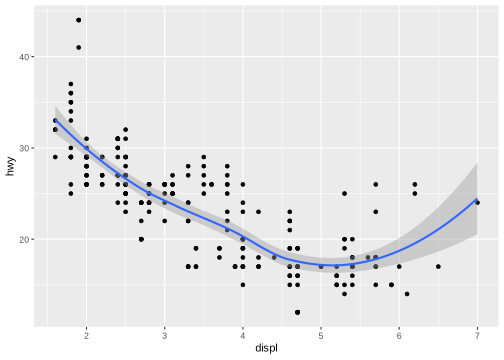
\includegraphics{template-computo-R_files/figure-pdf/pressure-1.pdf}

}

\end{figure}

It is also possible to create figures from static images:

\begin{figure}

{\centering 

\includegraphics[width=\textwidth,height=2.08333in]{template-computo-R_files/mediabag/logo_text_vertical.svg}

}

\caption{\label{fig-logo}Computo logo (label)}

\end{figure}

\hypertarget{tables}{%
\subsection{Tables}\label{tables}}

Tables (with label: \texttt{@tbl-mylabel} renders
Table~\ref{tbl-mylabel}) can be generated with markdown as follows

\hypertarget{tbl-mylabel}{}
\begin{longtable}[]{@{}lcr@{}}
\caption{\label{tbl-mylabel}my table caption}\tabularnewline
\toprule()
Tables & Are & Cool \\
\midrule()
\endfirsthead
\toprule()
Tables & Are & Cool \\
\midrule()
\endhead
col 1 is & left-aligned & \$1600 \\
col 2 is & centered & \$12 \\
col 3 is & right-aligned & \$1 \\
\bottomrule()
\end{longtable}

Table can also be generated by some code, for instance with knitr here:

\begin{Shaded}
\begin{Highlighting}[]
\NormalTok{knitr}\SpecialCharTok{::}\FunctionTok{kable}\NormalTok{(}\FunctionTok{summary}\NormalTok{(cars), }\AttributeTok{caption =} \StringTok{"Table caption."}\NormalTok{)}
\end{Highlighting}
\end{Shaded}

\begin{longtable}[]{@{}lll@{}}
\caption{Table caption.}\tabularnewline
\toprule()
& speed & dist \\
\midrule()
\endfirsthead
\toprule()
& speed & dist \\
\midrule()
\endhead
& Min. : 4.0 & Min. : 2.00 \\
& 1st Qu.:12.0 & 1st Qu.: 26.00 \\
& Median :15.0 & Median : 36.00 \\
& Mean :15.4 & Mean : 42.98 \\
& 3rd Qu.:19.0 & 3rd Qu.: 56.00 \\
& Max. :25.0 & Max. :120.00 \\
\bottomrule()
\end{longtable}

\hypertarget{sec-references}{%
\subsection{Handling references}\label{sec-references}}

\hypertarget{bibliographic-references}{%
\subsubsection{Bibliographic
references}\label{bibliographic-references}}

References are displayed as footnotes using
\href{http://www.bibtex.org/}{BibTeX}, e.g.~\texttt{{[}@computo{]}} will
be displayed as (Computo Team 2020), where \texttt{computo} is the
bibtex key for this specific entry. The bibliographic information is
automatically retrieved from the \texttt{.bib} file specified in the
header of this document (here: \texttt{references.bib}).

\hypertarget{other-cross-references}{%
\subsubsection{Other cross-references}\label{other-cross-references}}

As already (partially) seen, Quarto includes a mecanism similar to the
bibliographic references for sections, equations, theorems, figures,
lists, etc. Have a look at
\href{https://quarto.org/docs/authoring/cross-references.html}{this
page}.

\begin{tcolorbox}[enhanced jigsaw, colbacktitle=quarto-callout-warning-color!10!white, rightrule=.15mm, opacityback=0, breakable, colback=white, toptitle=1mm, arc=.35mm, opacitybacktitle=0.6, leftrule=.75mm, title=\textcolor{quarto-callout-warning-color}{\faExclamationTriangle}\hspace{0.5em}{For more information}, bottomtitle=1mm, coltitle=black, left=2mm, bottomrule=.15mm, toprule=.15mm, titlerule=0mm]

\begin{itemize}
\item
  \href{https://computo.sfds.asso.fr/published-paper-tsne/}{The template
  available in the Computo Quarto extension} uses advanced features and
  the KnitR kernel (interactive plots and pseudocode).
\item
  \href{https://computo.sfds.asso.fr/published-paper-tsne/}{Check our
  mock version of the t-SNE paper} for a full and advanced example using
  the Jupyter kernel.
\item
  Also look at the previously published paper in Computo for even
  advanced examples.
\end{itemize}

\end{tcolorbox}

\hypertarget{references}{%
\section*{References}\label{references}}
\addcontentsline{toc}{section}{References}

\hypertarget{refs}{}
\begin{CSLReferences}{1}{0}
\leavevmode\vadjust pre{\hypertarget{ref-computo}{}}%
Computo Team. 2020. {``Computo: Reproducible Computational/Algorithmic
Contributions in Statistics and Machine Learning.''}

\leavevmode\vadjust pre{\hypertarget{ref-R-base}{}}%
R Core Team. 2020. \emph{R: A Language and Environment for Statistical
Computing}. Vienna, Austria: R Foundation for Statistical Computing.
\url{https://www.R-project.org/}.

\leavevmode\vadjust pre{\hypertarget{ref-R-reticulate}{}}%
Ushey, Kevin, JJ Allaire, and Yuan Tang. 2020. \emph{Reticulate:
Interface to Python}. \url{https://github.com/rstudio/reticulate}.

\end{CSLReferences}

\hypertarget{session-information}{%
\section*{Session information}\label{session-information}}
\addcontentsline{toc}{section}{Session information}

\begin{Shaded}
\begin{Highlighting}[]
\FunctionTok{sessionInfo}\NormalTok{()}
\end{Highlighting}
\end{Shaded}

\begin{tcolorbox}[boxrule=0pt, enhanced, borderline west={2pt}{0pt}{code-block-stdout-light}, interior hidden, frame hidden, breakable, sharp corners, grow to left by=-1em]

\begin{verbatim}
R version 4.2.2 Patched (2022-11-10 r83330)
Platform: x86_64-pc-linux-gnu (64-bit)
Running under: Ubuntu 22.04.1 LTS

Matrix products: default
BLAS:   /usr/lib/x86_64-linux-gnu/atlas/libblas.so.3.10.3
LAPACK: /usr/lib/x86_64-linux-gnu/lapack/liblapack.so.3.10.0

locale:
 [1] LC_CTYPE=en_US.UTF-8       LC_NUMERIC=C              
 [3] LC_TIME=fr_FR.UTF-8        LC_COLLATE=en_US.UTF-8    
 [5] LC_MONETARY=fr_FR.UTF-8    LC_MESSAGES=en_US.UTF-8   
 [7] LC_PAPER=fr_FR.UTF-8       LC_NAME=C                 
 [9] LC_ADDRESS=C               LC_TELEPHONE=C            
[11] LC_MEASUREMENT=fr_FR.UTF-8 LC_IDENTIFICATION=C       

attached base packages:
[1] stats     graphics  grDevices datasets  utils     methods   base     

other attached packages:
[1] ggplot2_3.4.0

loaded via a namespace (and not attached):
 [1] pillar_1.8.1     compiler_4.2.2   tools_4.2.2      digest_0.6.31   
 [5] jsonlite_1.8.4   evaluate_0.20    lifecycle_1.0.3  tibble_3.1.8    
 [9] gtable_0.3.1     nlme_3.1-162     lattice_0.20-45  mgcv_1.8-41     
[13] pkgconfig_2.0.3  rlang_1.0.6      Matrix_1.5-3     cli_3.6.0       
[17] yaml_2.3.7       xfun_0.37        fastmap_1.1.0    withr_2.5.0     
[21] dplyr_1.1.0      knitr_1.42       generics_0.1.3   vctrs_0.5.2     
[25] grid_4.2.2       tidyselect_1.2.0 glue_1.6.2       R6_2.5.1        
[29] fansi_1.0.4      rmarkdown_2.20   farver_2.1.1     magrittr_2.0.3  
[33] scales_1.2.1     htmltools_0.5.4  splines_4.2.2    colorspace_2.1-0
[37] renv_0.16.0      labeling_0.4.2   utf8_1.2.3       munsell_0.5.0   
\end{verbatim}

\end{tcolorbox}



\end{document}
